% !TeX spellcheck = en_GB
% \begin{figure}[h!]
% 	\centering
% 		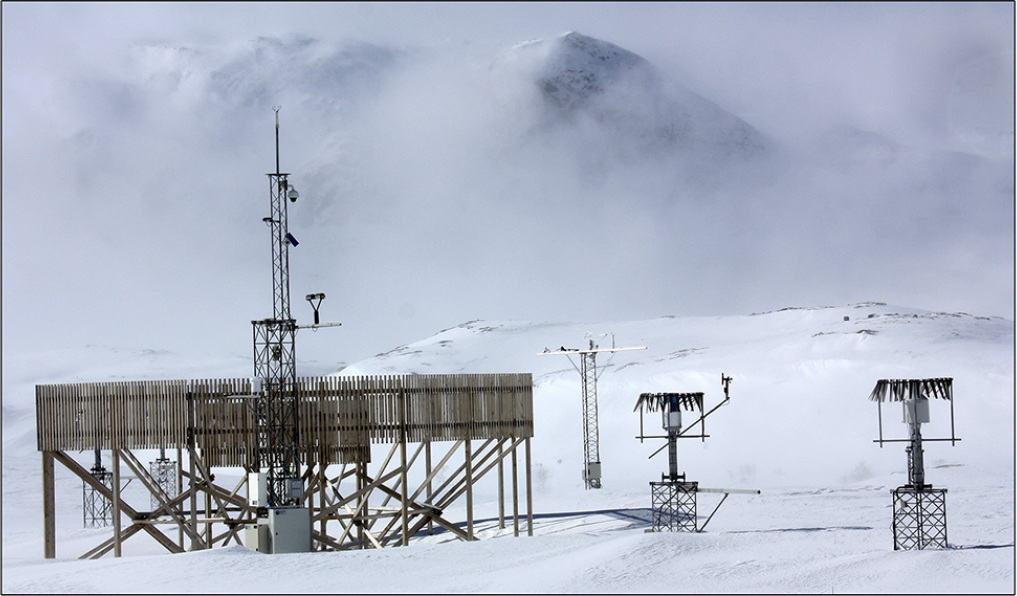
\includegraphics[width=0.55\textwidth]{./fig_instruments/Dofe.png}
% 	\caption{Picture, showing the double fence and unprotected precipitation gauges at the measurement site Haukeliseter. Picture taken from \cite{wolff_derivation_2015}.}\label{fig:Dofe}
% \end{figure}



\begin{wrapfigure}[28]{r}{0.44\textwidth}
	\vspace{-\normalbaselineskip}
	\centering
	\begin{subfigure}[b]{0.4\textwidth}
		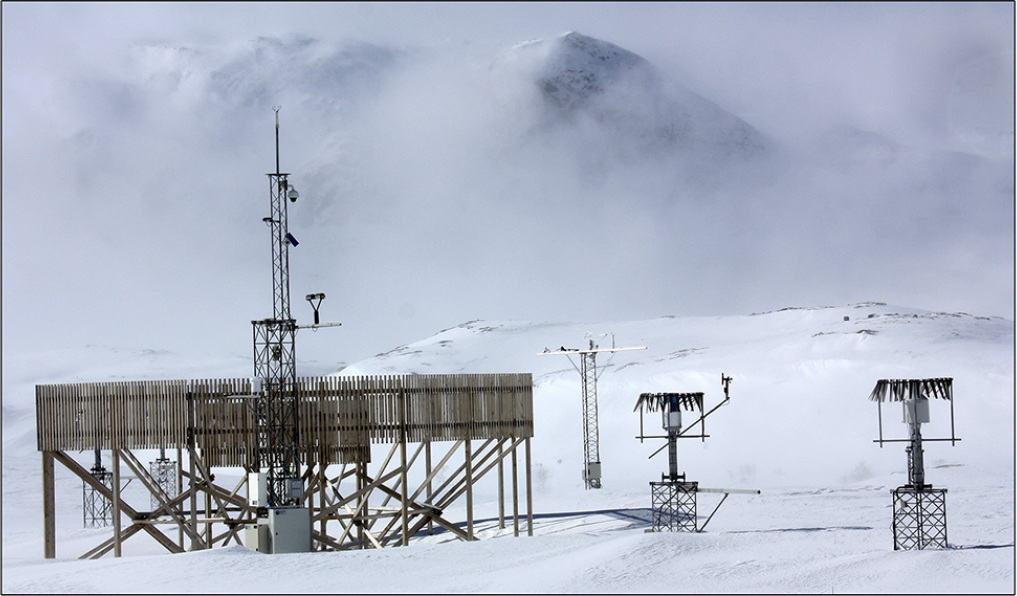
\includegraphics[width=\textwidth]{./fig_instruments/Dofe.png}
		\caption{}\label{fig:dofe_pic}
	\end{subfigure}	
	\begin{subfigure}[b]{0.4\textwidth}
		% 		\includegraphics[trim={0.8cm, 2.3cm, 2.4cm, 3cm},clip,width=1.1\textwidth]
		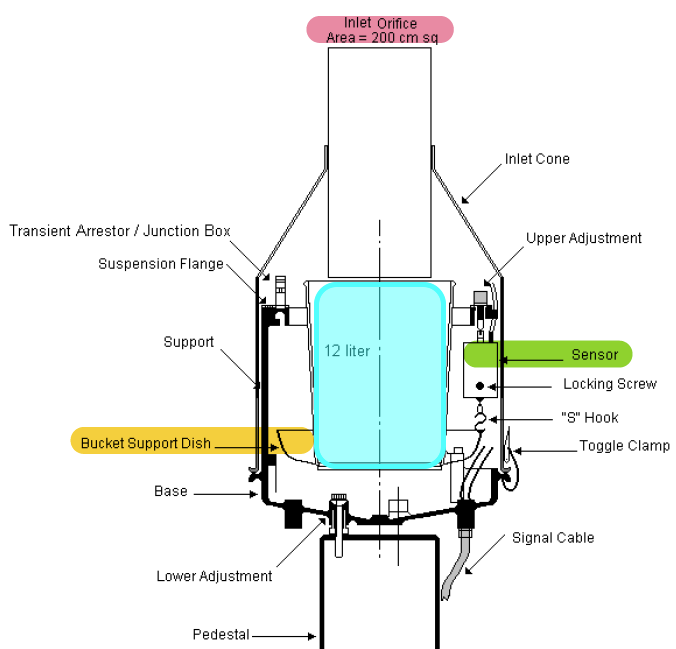
\includegraphics[width=1.1\textwidth]{./fig_instruments/Geonor_sketch2.png}
		\caption{}\label{fig:gauge_sketch}
	\end{subfigure}	
	\caption{(\protect\subref{fig:dofe_pic}) From left to right: Double fence gauge (\textbf{X0}) and unprotected precipitation gauges (\textbf{Nord, X4}) at Haukeliseter, from \cite{wolff_derivation_2015}. The prevailing easterly (westerly) wind from the lower, left corner in \protect\subref{fig:dofe_pic} (the opposite site). In front of the double fence gauge is the \SI{10}{\metre} weather mast (\textbf{M1}). (\protect\subref{fig:gauge_sketch}) Vertical cross section of Geonor T-200B3 precipitation gauge. pink: orifice; cyan: cylindric bucket with frost protection; yellow: bucket support dish; green: wire sensor \citep[adapted from][]{geonor_inc._t-200b_2015}.  }\label{fig:Dofe}
	%	\vspace{-\normalbaselineskip}
\end{wrapfigure}